% najpierw jest wstep, załączenie potrzebnych pakietów itp.
\documentclass[a4paper, 10pt]{article}

%polskie znaki
\usepackage[polish]{babel}
\usepackage[utf8]{inputenc}
\usepackage[OT4]{fontenc}
\usepackage{placeins}
%wieksze mozliwosci zmiany wygladu strony, pakiet do wstawiania linków
\usepackage{geometry}
\usepackage{ulem}
\RequirePackage{url}

% ladne wciecia akapitow i odstepy, mozna wykasowac wedle uznania;)
\setlength{\parindent}{0cm}
\setlength{\parskip}{3mm plus1mm minus1mm}

%mniejsze marginesy
\geometry{verbose,a4paper,tmargin=2.4cm,bmargin=2.4cm,lmargin=2.4cm,rmargin=2.4cm}
\usepackage{graphicx} % wstawianie obrazkow


%%%%%%%%%%%%%%%%%%%%%%%%%%%%%%%%%%%%%%%%%%%%%%%%

\title{{\bf {Metody odkrywania wiedzy }} \\ {\large Dokumentacja projektu}}
\date{\today}
\author{Dominika Sawicka \\Filip Nabrdalik}

%%%%%%%%%%%%%%%%%%%%%%%%%%%%%%%%%%%%%%%%%%%%%%%%
\begin{document}
\bibliographystyle{abbrv}
%%%%%%%
\null  % Empty line
\nointerlineskip  % No skip for prev line
\vfill
\let\snewpage \newpage
\let\newpage \relax
\maketitle %wstawienie tytulu, daty i autora
\let \newpage \snewpage
\vfill
\break % page break
%%%%%%%%%%%%%%%%%%%%%%%%%%%%%

\tableofcontents

\newpage


% Przydatne linki:
% 	http://www.ke.tu-darmstadt.de/lehre/archiv/ss12/web-mining/wm-tm.pdf
%	http://www.dis.uniroma1.it/~leon/didattica/webir/IR11.pdf
%	http://cran.r-project.org/web/packages/tm/tm.pdf
%	https://en.wikibooks.org/wiki/Data_Mining_Algorithms_In_R/Classification
%	http://www.statsoft.com.pl/textbook/stathome_stat.html?http%3A%2F%2Fwww.statsoft.com.pl%2Ftextbook%2Fstnaiveb.html




\section{Treść zadania}

{\bf{Zadanie 17}}

{\it Proste algorytmy klasyfikacji tekstu (TF-IDF, naiwny klasyfikator Bayesowski, kNN). Porównania ze standardowymi algorytmami klasyfikacji dostępnymi w R.}


\section{Algorytmy}
	\subsection{Autorskie algorytmy}
	{\bf{TF-IDF}}

TF-IDF (ang. TF – term frequency, IDF – inverse document frequency) informuje o częstości wystąpienia termów uwzględniając 
wyważenie znaczenia lokalnego termu oraz jego znaczeniu w kolekcji dokumentów. W algorytmie TF-IDF każdy dokument reprezentowany
jest przez wektor zawierający wagi słów występujących w dokumencie. Wartość TF-IDF (1):


\begin{equation}
\mathrm{(tf\mbox{-}idf)_{i,j}} = \mathrm{tf_{i,j}} \times  \mathrm{idf_{i}}
\end{equation}

"Term frequency" (2), gdzie $n_{i,j}$ to liczbą wystąpień termu ($t_{i}$) w dokumencie $d_{j}$, a mianownik jest sumą liczby wystąpień wszystkich termów w dokumencie $d_{j}$:
 
\begin{equation}
\mathrm{tf_{i,j}} = \frac{n_{i,j}}{\sum_k n_{k,j}}
\end{equation}

"Inverse document frequency" (3), gdzie $|D|$ to liczba dokumentów, a $|\{d : t_{i} \in d\}|$ reprezentuje zbiór dokumentów zawierających
jedno wystąpienie danego termu:

\begin{equation}
\mathrm{idf_{i}} =  \log \frac{|D|}{|\{d: t_{i} \in d\}|}
\end{equation}

W autorskiej wersji algorytmu TF-IDF służy do przygotowania danych, natomiast do klasyfikacji jest używany kNN.



{\bf{kNN}}

Algorytm kNN (ang. k-nearest neighbors algorithm) pozwala sklasyfikować nieznany dokument $X$  poprzez uszeregowanie sąsiadów dokumentu spośród wektorów treningowych i 
wykorzystanie przynależności do klas $k$ najbardziej podobnych sąsiadów do przewidzenia klasy nieznanego dokumentu. Klasom sąsiadów przypisuje się wagi w zależności od 
podobieństwa każdego sąsiada do $X$ mierzonego odległością euklidesową lub wartością cosinusa kąta pomiędzy opisującymi je wektorami ważonych atrybutów. 
Podobieństwo mierzone wartością cosinusa definiuje następujący wzór:

\begin{equation}
\mathrm{sim(X, D_{j}) = \frac{
\sum_{ t_{i} \in (x\cap D_{j})
  }x_{i} \times d_{ij}}{||X||_{2} \times ||D_{j}||_{2}}}
\end{equation}

gdzie:\\
$X$ - testowany dokument reprezentowany w postaci wektora\\
$D_{j}$ - $j$-ty dokument treningowy\\
$t_{i}$ - słowo wspólne dla $X$ i $D_{j}$\\
$x_{i}$ - waga słowa $t_{i}$ w $X$\\
$d_{ij}$ - waga słowa $t_{i}$ w dokumencie $D_{j}$\\
$||X||_{2} = \sqrt{{x_{1}}^{2} + {x_{2}}^{2} + {x_{3}}^{2} + ...}$ - norma X\\
$||D_{j}||_{2}$ - norma $D_{j}$\\

Podobieństwo w autorskiej wersji algorytmu knn określa się za pomocą odległości euklidesowej.


%http://www.mimuw.edu.pl/~krzadca/zadanie-kNN.html

{\bf{Naiwny klasyfikator bayesowski}}

Naiwny klasyfikator bayesowski (1) jest to prosty klasyfikator probabilistyczny, którego w trybie "uczenia z nadzorem" można skutecznie użyć do 
klasyfikacji dokumentów.

\begin{equation}
p(C \vert F_1,\dots,F_n) = \frac{1}{Z}  p(C) \prod_{i=1}^n p(F_i \vert C)
\end{equation}

Powyższego wzoru (4), wynikającego z tw. Bayesa, można użyć do zaklasyfikowania dokumentu do danego zbioru lub klasy jeśli spełniony jest warunek (6).
\begin{equation}
\ln{p(S\vert D)\over p(\neg S\vert D)}=\ln{p(S)\over p(\neg S)}+\sum_i \ln{p(w_i\vert S)\over p(w_i\vert\neg S))}
\end{equation}
\begin{equation}
\ln{p(S\vert D)\over p(\neg S\vert D)} > 0
\end{equation}

Gdzie: $S$ - klasa dokumentu, $D$ - dokumenty, $w_i$ - pojedynczy term lub słowo.
	

	\subsection{Standardowe algorytmy klasyfikacji tekstu w R}
	
	{\bf{Naiwny klasyfikator bayesowski w R}}
	
	Do badań została wykorzystana implementacja algorytmu z pakietu $e1071$. Niestety brak czasu uniemożliwił jego poprawną implementację. Jego kod został załączony 
	do sprawozdania, lecz wyniki są pominięte na wykresach.
	
	
	{\bf{kNN w R}}
	
	Do badań została wykorzystana implementacja algorytmu z pakietu $class$.
	
	{\bf{SVM w R}}
	
	Klasyfikator, którego nauka ma na celu wyznaczenie hiperpłaszczyzny rozdzielającej z maksymalnym marginesem przykłady należące do dwóch klas.
	Do badań została wykorzystana implementacja algorytmu z pakietu $e1071$.
	
	{\bf{Random Forest w R}}
	
	Algorytm oparty o tworzenie lasów drzew decyzyjnych podczas nauki do klasyfikacji. Do badań została wykorzystana implementacja algorytmu z pakietu $randomForest$.
	
	

\section{Eksperymenty badawcze}


Jakość modeli jest oceniana przy pomocy dwóch parametrów $precision$ oraz $recall$. Dodatkowym 
parametrem uwzględnionym w wynikach badań jest czas wykonania poszczególnych klasyfikatorów. 
W celu zwiększenia wiarygodności badań, każdy eksperyment powtarzany był 5 razy, a uzyskane wyniki prezentowane 
są w uśrednionej postaci. W celu miarodajnego porównania klasyfikatorów wykonane zostały eksperymenty dla różnych wielkości 
zbiorów danych trenujących i testowych. Testy są w pełni zautomatyzowane, aby rozpocząć procedurę testowa należy uruchomić skrypt 
$run.r$.






	\subsection{Charakterystyka zbiorów danych}
	
Do celów testowych wykorzystane zostały następujace zbiory danych z repozytorium UCI.\\

\textbf{SMS Spam} \url{(http://archive.ics.uci.edu/ml/datasets/SMS+Spam+Collection)} \\ kolekcja ponad 5000 Wiadomości SMS w języku angielskim, z których ok. 1000 zawiera spam. Dane zebrane są w jednym pliku, każda wiadomość znajduje się oddzielnym wierszu i 
jest poprzedzona informacja do jakiego typu należy. Dane te są wykorzystywane w eksperymentach algorytmu TF-IDF oraz w obu wersjach naiwnego klasyfikatora bayesowskiego. \\

\textbf{SpamBase} (\url{http://archive.ics.uci.edu/ml/datasets/Spambase}) \\ zbiór przykładów wygenerowany z 4601 Wiadomości email z których ok. 40\% została zaklasyfikowana jako spam. Atrybuty zostały otrzymane z 48 najczęściej występujących słów, 
6 ze znaków specjalnych i~interpunkcyjnych oraz 3 z ilości nieprzerwanych ciągów wielkich liter.  Każdy wiersz zawiera następujące atrybuty: 54 całkowitoliczbowych $[1,100]$ procent występowania słowa lub znaku w danej wiadomości 
i 3 całkowitoliczbowe reprezentujące ilość wielkich liter oraz średnia i maksymalna długość łańcuchów wielkich liter w danej wiadomości email. Ostatni atrybut w zbiorze danych wskazuje czy dana wiadomość jest spamem. 
Dane nie wymagają dalszej obróbki i zostały wykorzystane podczas badań 	algorytmów kNN, SVM, random forest oraz autorskiej wersji kNN.
	
	
	\subsection{Parametry algorytmów}
W eksperymentach badawczych zostały uwzględnione 3 wersje algorytmu kNN w zależności od parametru $k=(3,6,12)$.


	\subsection{Sposób oceny jakości modeli}
	
	Do oceny modeli użyliśmy parametru F-score, który jest średnia harmoniczną parametrów $precision$ i $recall$.
	
	
\begin{equation}
recall = \frac{TP}{TP + FN}
\end{equation}

\begin{equation}
precision = \frac{TP}{FP + TP}
\end{equation}

\begin{equation}
{F-score} = \frac{2*precision*recall}{precision + recall}
\end{equation}


gdzie:\\
$TP$ (true positive) - wiadomości będące SPAMem, zaklasyfikowane jako SPAM\\
$FP$ (false positive) - wiadomości będące SPAMem, nie zaklasyfikowane jako SPAM\\
$FN$ (false negative) - wiadomości nie będące SPAMem, zaklasyfikowane jako SPAM\\

	


\subsection{Uwagi do eksperymentów}

Długi czas obliczeń dla TF-IDF umożliwił zrealizowanie tylko części eksperymentów z jego udziałem.
W sprawozdaniu zostały opisane następujące eksperymenty.

\begin{itemize}
  \item Czas klasyfikacji dla 10 przykładów, dla liczności zbioru trenującego odpowiednio $(100,150,300,500)$
  \item F-score dla 10 przykładów, dla liczności zbioru trenującego odpowiednio $(100,150,300,500)$
  \item F-score dla liczności zbioru trenującego odpowiednio $L=(100,150,300,500,1000)$ i ilości przykładów do klasyfikacji $0.25*L_i$
  \item F-score dla liczności zbioru trenującego odpowiednio $L=(100,150,300,500,1000)$ i ilości przykładów do klasyfikacji $0.5*L_i$. Bez TF-IDF.
  \item F-score dla liczności zbioru trenującego odpowiednio $L=(50,75,150,250,500)$ i ilości przykładów do klasyfikacji $2*L_i$. Bez TF-IDF.
\end{itemize}





\section{Wyniki}

\begin{figure}[ht!]
\centering
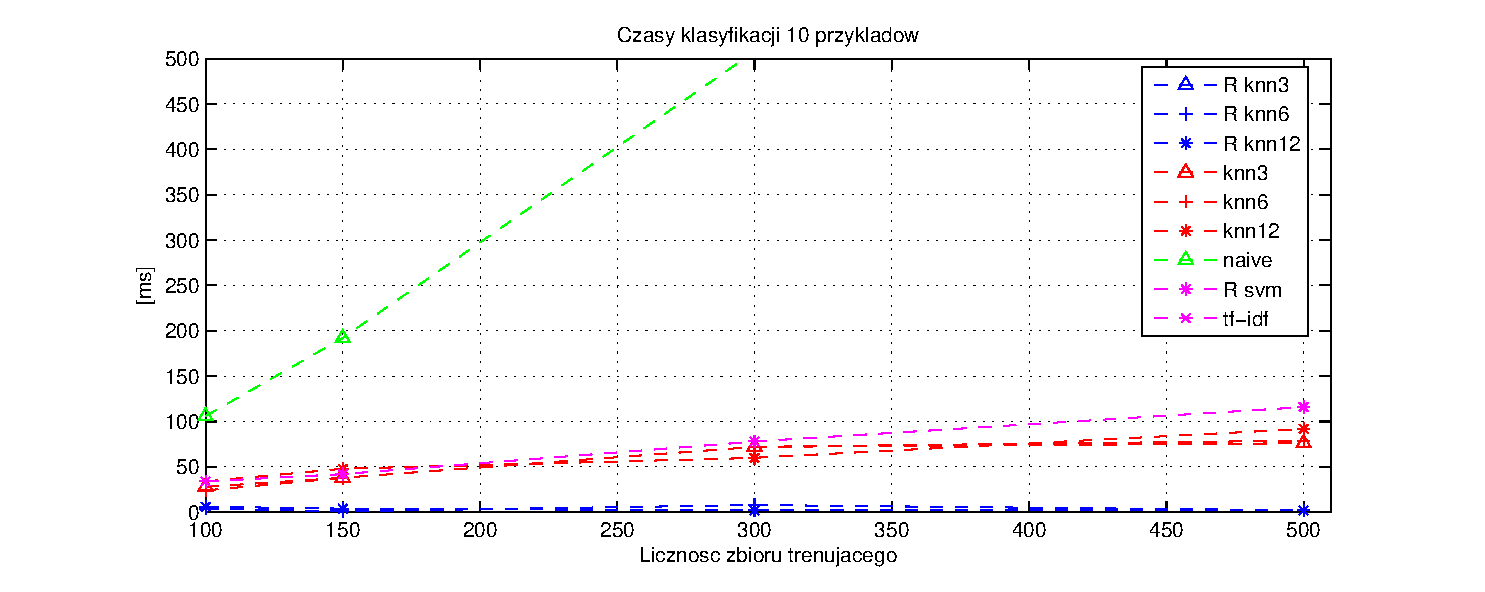
\includegraphics[width=165mm]{wykresy/czas500.eps}
\caption{\it{Czasy zaklasyfikowania 10 przykładów, TF-IDF oraz naiwny klasyfikator bayesowski nie mieści się w skali}}
\label{overflow}
\end{figure}

\begin{figure}[ht!]
\centering
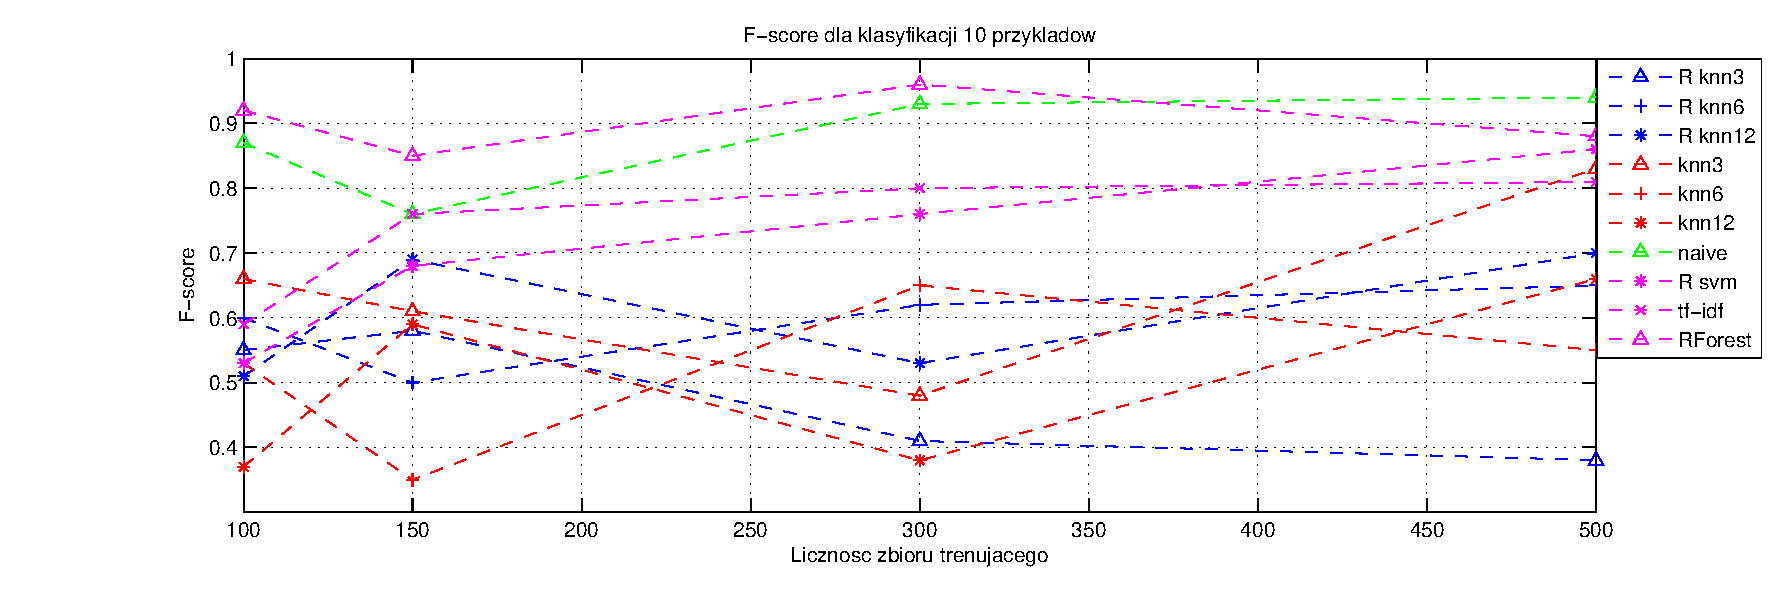
\includegraphics[width=165mm]{wykresy/score500.eps}
\caption{\it{F-score dla zaklasyfikowania 10 przykładów, $L=(100,150,300,500)$}}
\label{overflow}
\end{figure}

\begin{figure}[ht!]
\centering
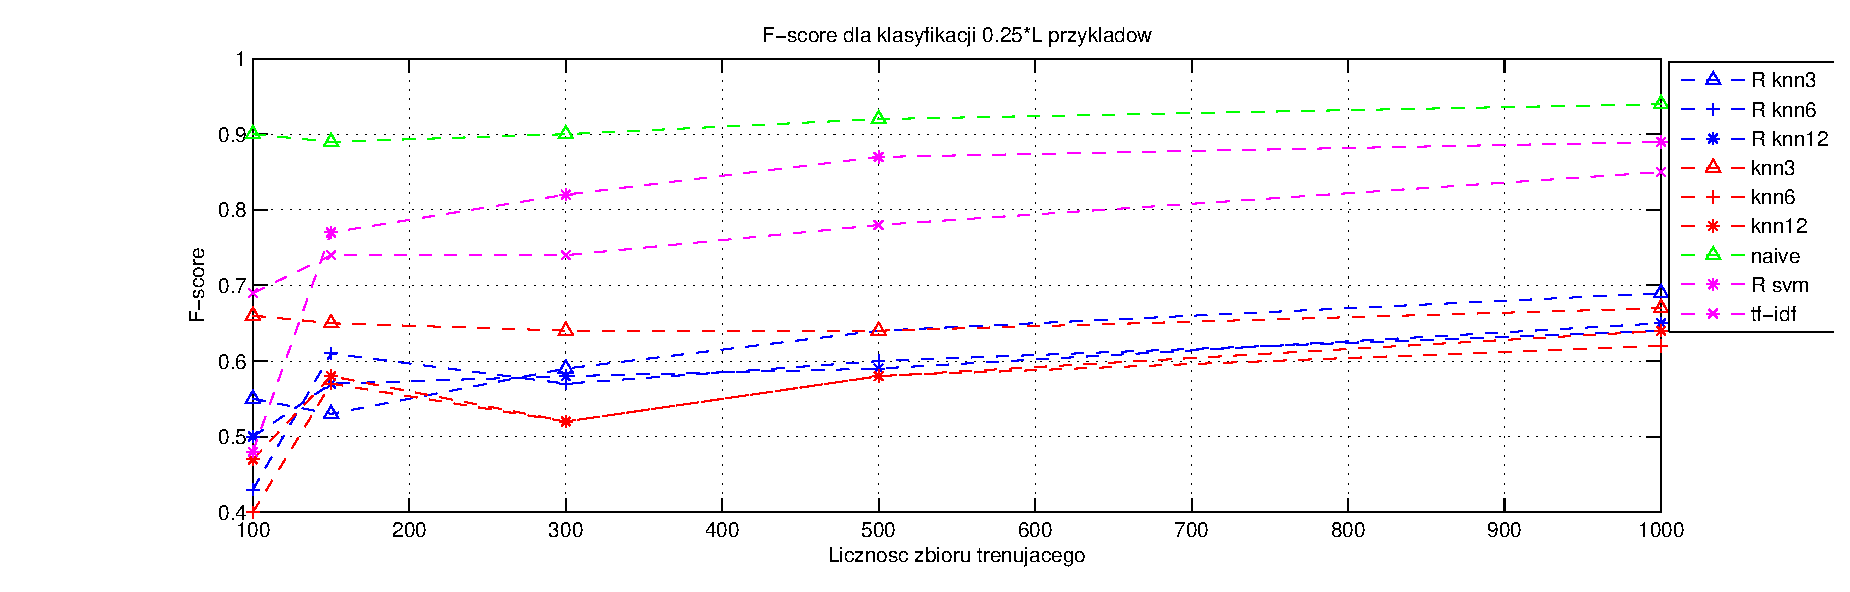
\includegraphics[width=165mm]{wykresy/score1000.eps}
\caption{\it{F-score dla zaklasyfikowania $0.25*L_i$ przykładów, $L=(100,150,300,500,1000)$}}
\label{overflow}
\end{figure}

\begin{figure}[ht!]
\centering
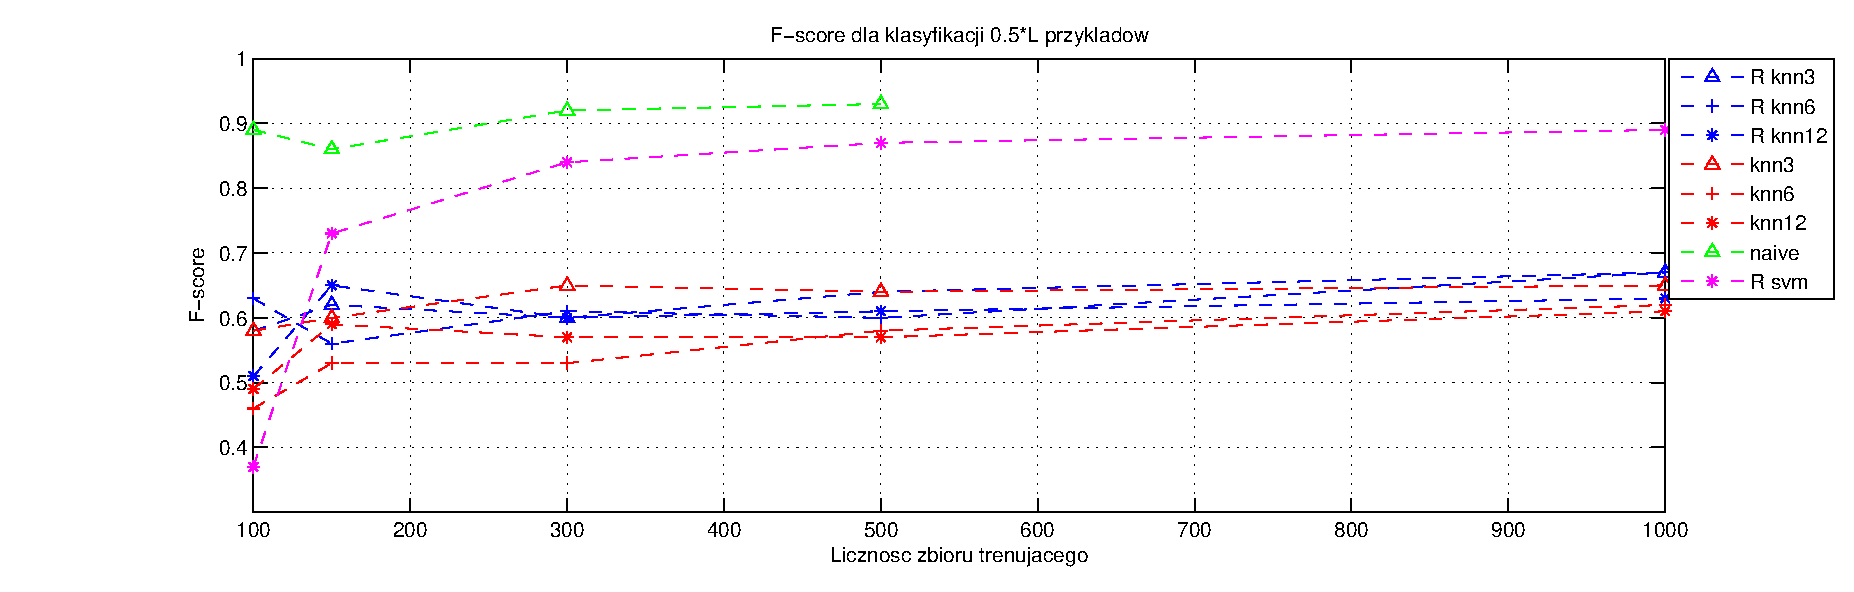
\includegraphics[width=165mm]{wykresy/score1000-05.eps}
\caption{\it{F-score dla zaklasyfikowania $0.5*L_i$ przykładów, $L=(100,150,300,500,1000)$. Bez TF-IDF.}}
\label{overflow}
\end{figure}

\begin{figure}[ht!]
\centering
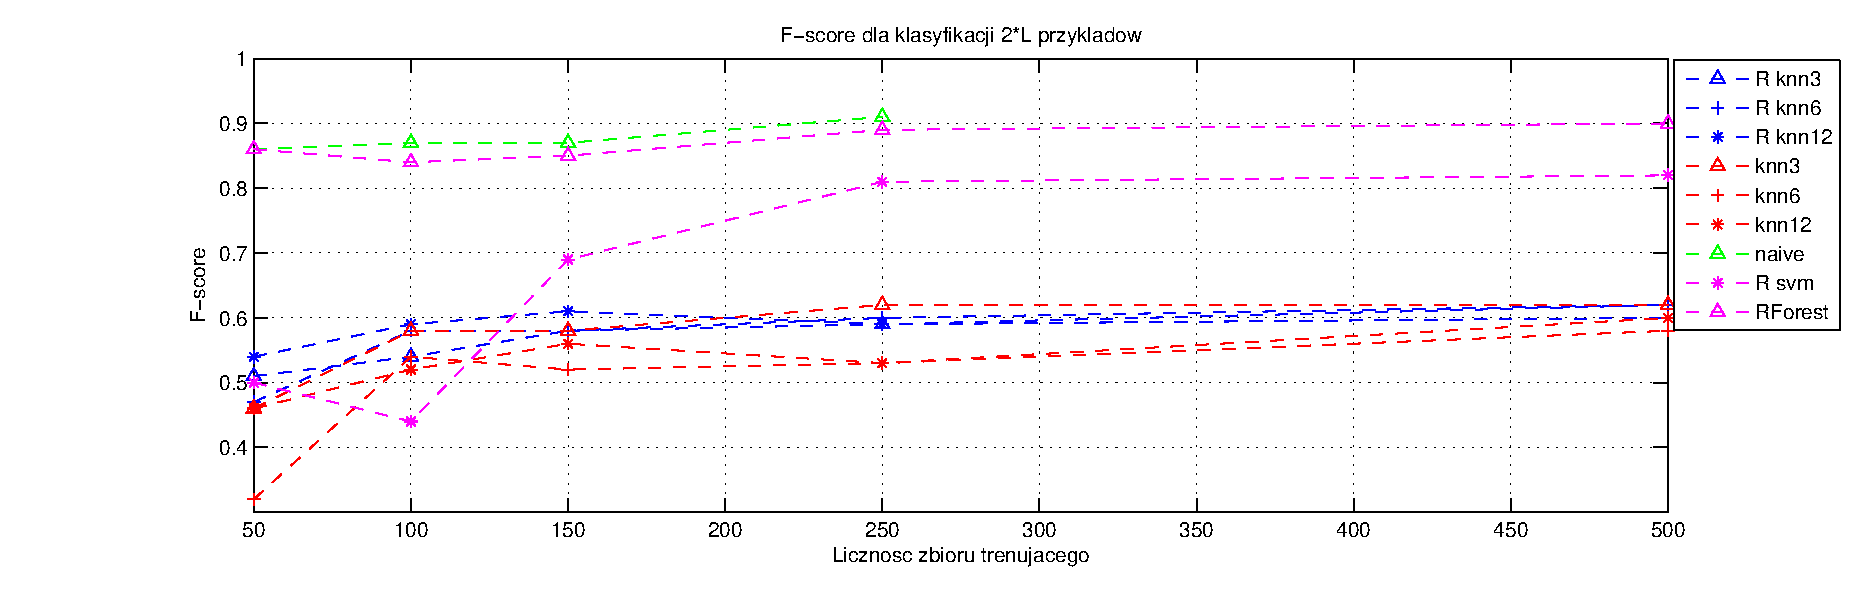
\includegraphics[width=165mm]{wykresy/score500-2.eps}
\caption{\it{F-score dla zaklasyfikowania $2*L_i$ przykładów, $L=(50,75,150,250,500)$. Bez TF-IDF.}}
\label{overflow}
\end{figure}

\FloatBarrier

\section{Wnioski}

\subsection{Interpretacja wyników}

\subsection{Odpowiedzi na pytania}
\begin{itemize}
\item{Który z testowanych algorytmów klasyfikacji jest najlepszy w kontekście badanych parametrów?}
\item{Jak rozmiar danych uczących wpływa na poprawę skuteczności modeli?}
\item{Czy na podstawie przeprowadzonych testów możliwe jest wyłonienie bezwzględnie najlepszego algorytmu?}
\end{itemize}





%BIBLIOGRAFIA
\nocite{*}
\bibliography{bibliografia}


\end{document}


